\documentclass[border=10pt]{standalone}
\usepackage[svgnames]{xcolor}
\usepackage{amsmath}
\usepackage{pgfplots}
\pgfplotsset{compat=newest}
\usepackage[sfdefault]{FiraSans}
\usepackage{FiraMono}
\renewcommand*\familydefault{\sfdefault}
\begin{document}
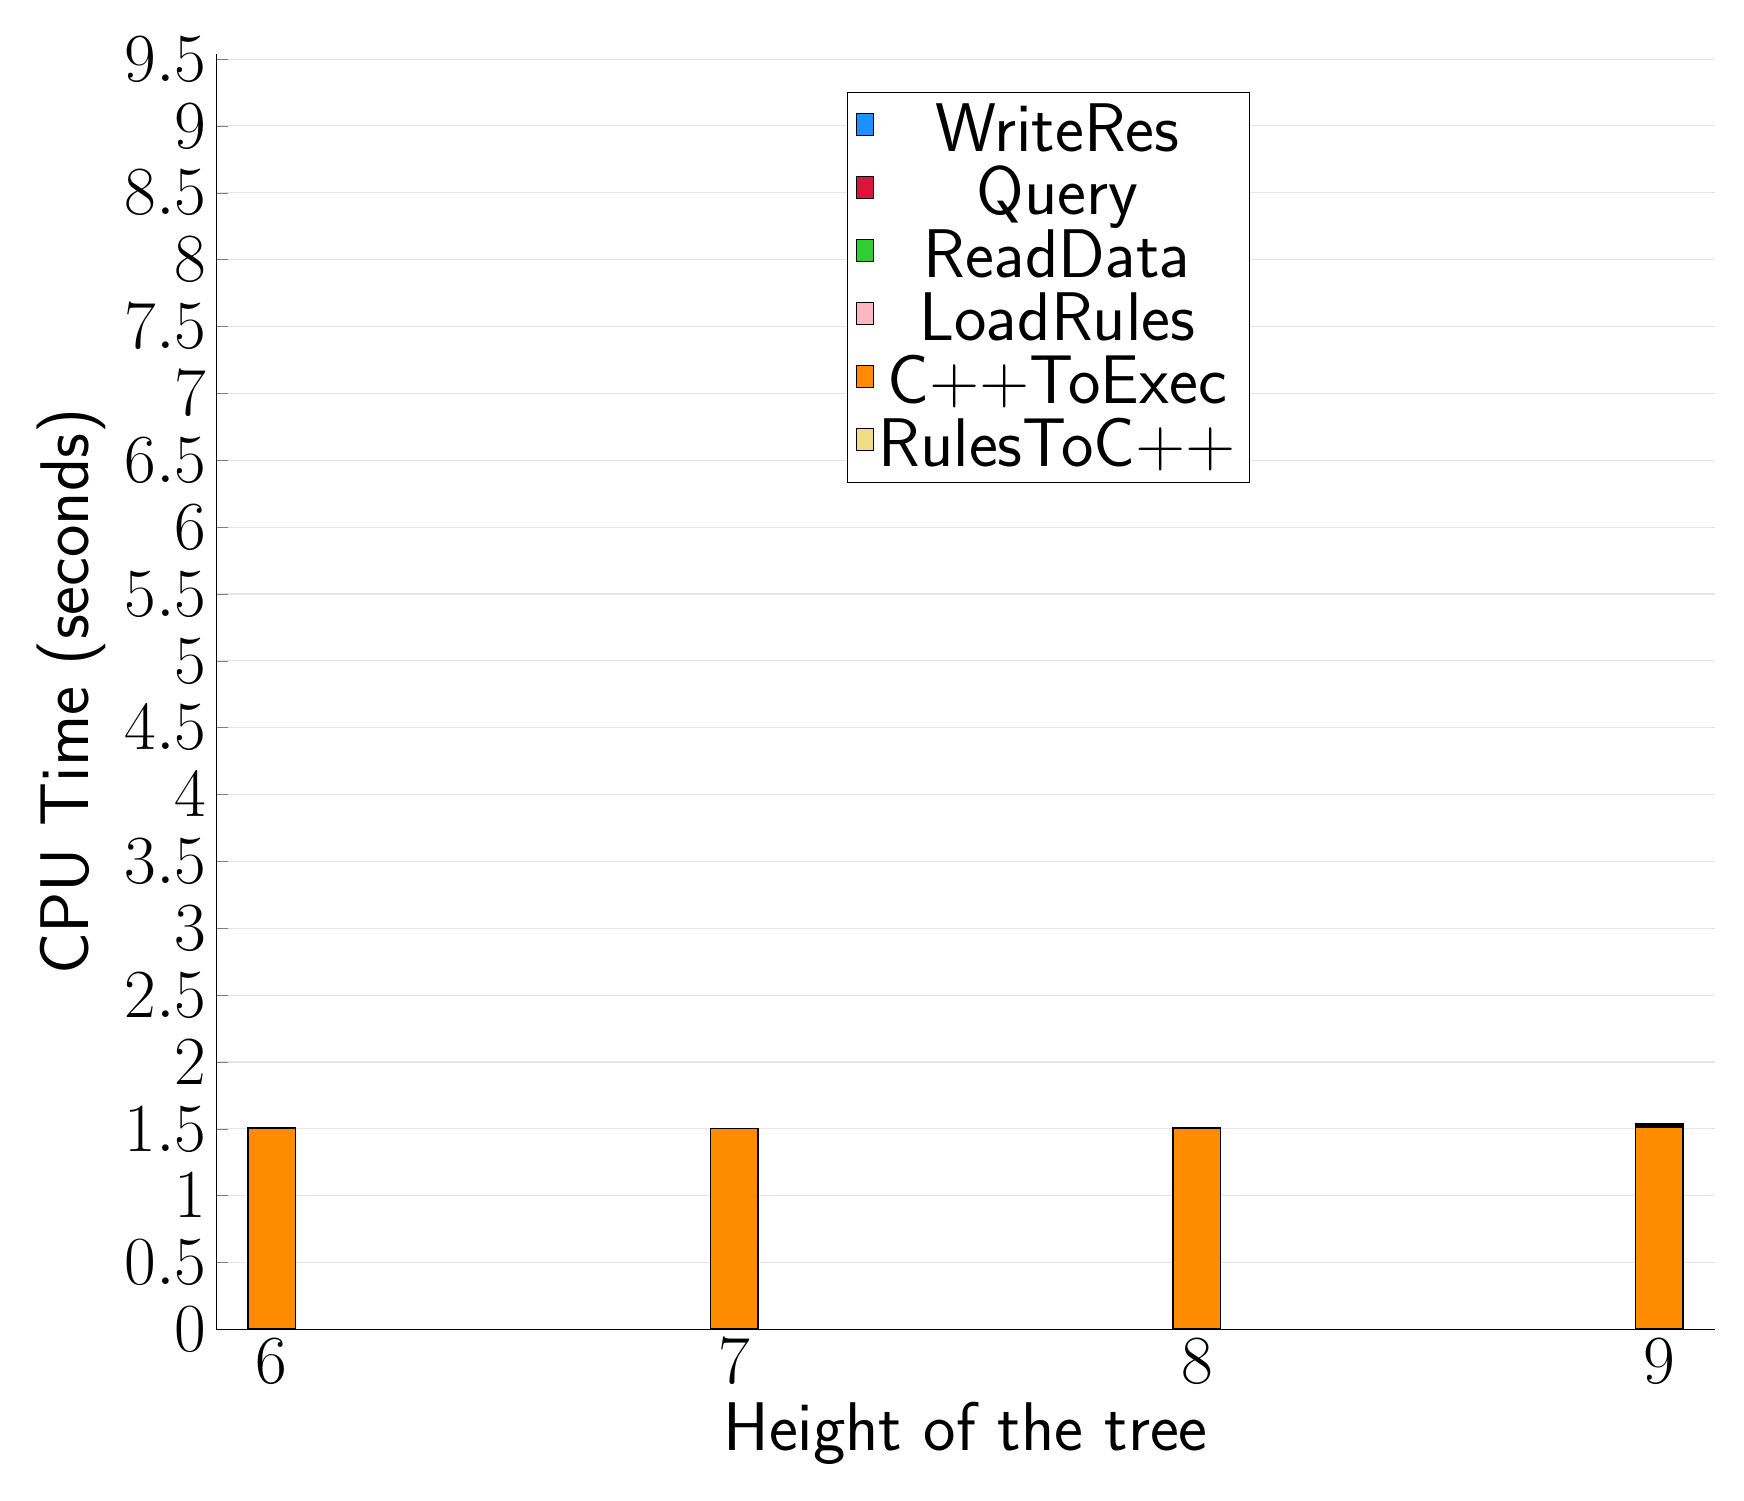
\begin{tikzpicture}
\begin{axis}[
   ybar stacked,
   width=1.7\textwidth,
   bar width=0.6cm,
   ymajorgrids, tick align=inside,
   major grid style={draw=gray!20},
   xtick=data,
   ymin=0, ymax=9.538,
   axis x line*=bottom,
   axis y line*=left,
   enlarge x limits=0.04,
   legend style={
       at={(0.69, 0.97)},
       anchor=north east,
       legend columns=1,
       font=\Huge,
   },
   ylabel={CPU Time (seconds)},
   xlabel={Height of the tree},
   label style={font=\Huge},
   tick label style={font=\Huge},
]
\addlegendimage{fill=DodgerBlue, draw=black, line width=0.2pt}
\addlegendentry{WriteRes}
\addlegendimage{fill=Crimson, draw=black, line width=0.2pt}
\addlegendentry{Query}
\addlegendimage{fill=LimeGreen, draw=black, line width=0.2pt}
\addlegendentry{ReadData}
\addlegendimage{fill=LightPink, draw=black, line width=0.2pt}
\addlegendentry{LoadRules}
\addlegendimage{fill=DarkOrange, draw=black, line width=0.2pt}
\addlegendentry{C++ToExec}
\addlegendimage{fill=LightGoldenrod, draw=black, line width=0.2pt}
\addlegendentry{RulesToC++}
\addplot +[fill=LightGoldenrod, draw=black, line width=0.55pt] coordinates {
(6, 0.0020000000000000005)
(7, 0.0020000000000000005)
(8, 0.0020000000000000005)
(8, 0.0)
(8, 0.0020000000000000005)
(9, 0.004000000000000001)
(9, 0.0)
(9, 0.0)
(9, 0.0020000000000000005)
(9, 0.0)
};
\addplot +[fill=DarkOrange, draw=black, line width=0.55pt] coordinates {
(6, 1.5059999999999998)
(7, 1.5)
(8, 1.502)
(8, 1.5059999999999998)
(8, 1.5059999999999998)
(9, 1.51)
(9, 1.5279999999999998)
(9, 1.5240000000000002)
(9, 1.5240000000000002)
(9, 1.532)
};
\addplot +[fill=LightPink, draw=black, line width=0.55pt] coordinates {
(6, 0.0001498)
(7, 0.00011399999999999999)
(8, 7.539999999999999e-05)
(8, 9.760000000000001e-05)
(8, 0.000117)
(9, 0.00010780000000000002)
(9, 0.00014099999999999998)
(9, 0.00014399999999999998)
(9, 0.0001512)
(9, 0.000152)
};
\addplot +[fill=LimeGreen, draw=black, line width=0.55pt] coordinates {
(6, 0.0006475999999999999)
(7, 0.0006676000000000001)
(8, 0.0009078000000000001)
(8, 0.0010134)
(8, 0.0009916)
(9, 0.0013936)
(9, 0.0024098)
(9, 0.0024209999999999995)
(9, 0.002291)
(9, 0.0024795999999999998)
};
\addplot +[fill=Crimson, draw=black, line width=0.55pt] coordinates {
(6, 0.0005064)
(7, 0.0009165999999999998)
(8, 0.0021666)
(8, 0.0021225999999999997)
(8, 0.0022443999999999997)
(9, 0.004402400000000001)
(9, 0.0064566)
(9, 0.006612799999999999)
(9, 0.0061038)
(9, 0.006495799999999999)
};
\addplot +[fill=DodgerBlue, draw=black, line width=0.55pt] coordinates {
(6, 0.0001386)
(7, 7.18e-05)
(8, 8.539999999999999e-05)
(8, 7.34e-05)
(8, 0.0001238)
(9, 6.039999999999999e-05)
(9, 0.00015719999999999997)
(9, 0.0001608)
(9, 0.0001394)
(9, 0.0001504)
};
\end{axis}
\end{tikzpicture}

\end{document}
